\documentclass[a4paper,12pt]{article}
\usepackage[utf8]{inputenc}         % кодировка исходного текста
\usepackage[russian]{babel} % локализация и переносы

\usepackage{amsmath, amssymb, amsthm, graphicx, epsfig, fancyhdr}
\usepackage{cmap}                   % поиск в PDF


%%% Дополнительная работа с математикой
\usepackage{amsmath,amsfonts,amssymb,amsthm,mathtools, mathabx} % AMS
\usepackage{icomma} % "Умная" запятая: $0,2$ --- число, $0, 2$ --- перечисление

%% Диаграммы XY-pic для редукционных графов
\usepackage[all]{xy}

\usepackage{hyperref}
\usepackage{graphicx}
%% Номера формул
\mathtoolsset{showonlyrefs=true} % Показывать номера только у тех формул, на которые есть \eqref{} в тексте.

%% Шрифты
\usepackage{euscript} 
\usepackage{mathrsfs} 

\usepackage{forloop}

% для сноски в виде символа, а не номера
\usepackage[symbol]{footmisc}
\renewcommand{\thefootnote}{\fnsymbol{footnote}}

% графики
\usepackage{tikz}
\newcommand{\LD}{\langle}
\newcommand{\RD}{\rangle}

\newcounter{zcounter}

\newcommand{\z}{\par\addtocounter{zcounter}{1}%
\textsc{\fbox{\textbf{FP\arabic{zcounter}}}\quad} }

\newcommand{\zopt}{\par\addtocounter{zcounter}{1}%
\textsc{\fbox{FP\arabic{zcounter}}\quad} }

\textwidth=175mm
\oddsidemargin=-8mm
\topmargin=-8mm

\makeatletter
\newcommand{\rmnum}[1]{\romannumeral #1}
\newcommand{\Rmnum}[1]{\expandafter\@slowromancap\romannumeral #1@}
\makeatother

\newcounter{symbcopy}
\newcommand{\nsymbl}[2]{
  \forloop{symbcopy}{0}{\value{symbcopy} < #2}{#1}
}

\newcommand{\eqdef}{\stackrel{\mathrm{def}}{=}}



\DeclareMathOperator{\true}{TRUE}
\DeclareMathOperator{\false}{FALSE}
\DeclareMathOperator{\sub}{SUB}
\DeclareMathOperator{\iszero}{isZero}
\DeclareMathOperator{\SUCC}{SUCC}
\DeclareMathOperator{\MULT}{MULT}
\DeclareMathOperator{\ADD}{ADD}
\DeclareMathOperator{\LE}{LE}
\DeclareMathOperator{\AND}{AND}
\DeclareMathOperator{\PREV}{PREV}


\title{Функциональное программирование \\ Задание 2}
\author{ Кобылянский А.В. \\ Группа 5381 }
\date {}


\begin{document}
\pagenumbering{gobble}
\maketitle
\newpage
\pagenumbering{arabic}

\z Реализуйте для чисел Чёрча следующие функции:
\break

$\bullet \:$ вычитания;

Так как нумералы Черча неотрицательны, то определим ``вычитание'' как 
$$
    a \dotdiv b =  \begin{cases} a - b, & \mbox{if } a > b \\ 0, & \mbox{if } a \le b \end{cases}
$$

Тогда 
$$
    \sub \equiv \lambda ab.b \: \operatorname{PREV} \: a
$$

$\bullet \:$ проверки на равенство;

Из определения
$$
    a \dotdiv b = 0 \iff a \le b
$$

Мы можем вывести условие для равенства
$$
    a \dotdiv b = 0 \land b \dotdiv a = 0 \iff a \le b \land b \le a \iff a = b
$$

Тогда
\begin{align*}
    \iszero &\equiv \lambda n. n \: (\lambda x . \false) \: \true \\
    \LE &\equiv \lambda ab. \iszero(\sub a \: b) \\
    \AND &\equiv \lambda ab. a \: b \: \false \\
    \operatorname{isEquile} &\equiv \lambda ab. \operatorname{AND} \:
    (\LE a \: b) \: (\LE b \: a)
\end{align*}
\hfill\break

\z Постройте замкнутый $\lambda$-терм \textit{в нормальной форме}, представляющий функцию
\[f(n) = 2n^2 + 3n + 1\]
для чисел Чёрча.
\hfill\break

Преобразуем наше выражение к виду $(n + 1)(2n + 1)$, тогда
\begin{align*}
    \SUCC &\equiv \lambda n s z. s(nsz) \\
    \ADD &\equiv \lambda nmsz. ns(msz) \\
    \MULT &\equiv \lambda nms. n(ms) \\
    f(n) &\equiv \lambda n . \MULT \: (\SUCC n) \: (\SUCC (\ADD n \: n)) \\
    &=_\beta \lambda n . \MULT \: (\lambda s z. s(nsz)) \: (\SUCC (\ADD n \: n)) \\
    &=_\beta \lambda n . \MULT \: (\lambda s z. s(nsz)) \: (\SUCC (\lambda sz. ns(nsz))) \\
    &\equiv \lambda n . \MULT \: (\lambda s z. s(nsz)) \: ((\lambda n s z. s(nsz)) (\lambda sz. ns(nsz))) \\
    &=_\beta \lambda n . \MULT \: (\lambda s z. s(nsz)) \: \lambda s z. s(ns(nsz)))\\  
    &\equiv \lambda n . (\lambda nms. n(ms)) \: (\lambda s z. s(nsz)) \: \lambda s z. s(ns(nsz)))\\   
    &=_\beta \lambda n . \lambda s. (\lambda s z. s(nsz)) \: \lambda z. s(ns(nsz)) \\  
    &=_\beta \lambda n . \lambda s. \lambda z. [\lambda z'. s(ns(nsz'))](n[\lambda z'. s(ns(nsz'))]z)  \\    
    &=_\beta \lambda n . \lambda s. \lambda z. s(ns(ns(n[\lambda z'. s(ns(nsz'))]z))) 
\end{align*}
\hfill\break

\z Реализуйте функцию $map$, которая применяет переданную функцию к каждому элементу переданного списка. То есть
\[
map \: f \: [a, \: b, \: c] \: \Longrightarrow \: [f a, \: f b,\: f c]
\]
Список реализуйте через его функцию свертки. \\
Например, список $[a, \: b, \: c]$ становится функцией, которая принимает два аргумента $f$ и $z$ и возвращает $f \: a \: (f \: b \: (f \: c \: z))) $

\begin{align*}
    \operatorname{NIL} &\equiv \lambda fz. z \\ 
    \operatorname{CONS} &\equiv \lambda alfz. f \: a \: (l \: f \: z) \\ 
    \operatorname{MAP}  &\equiv \lambda gl. 
    l \: (\lambda x. \operatorname{CONS} \: (gx)) \operatorname{NIL}  
\end{align*}

\bigbreak

\z \href{https://en.wikipedia.org/wiki/Fibonacci_number}{Числа Фибоначчи} описывают идеализированную модель популяции кроликов.
\begin{center}
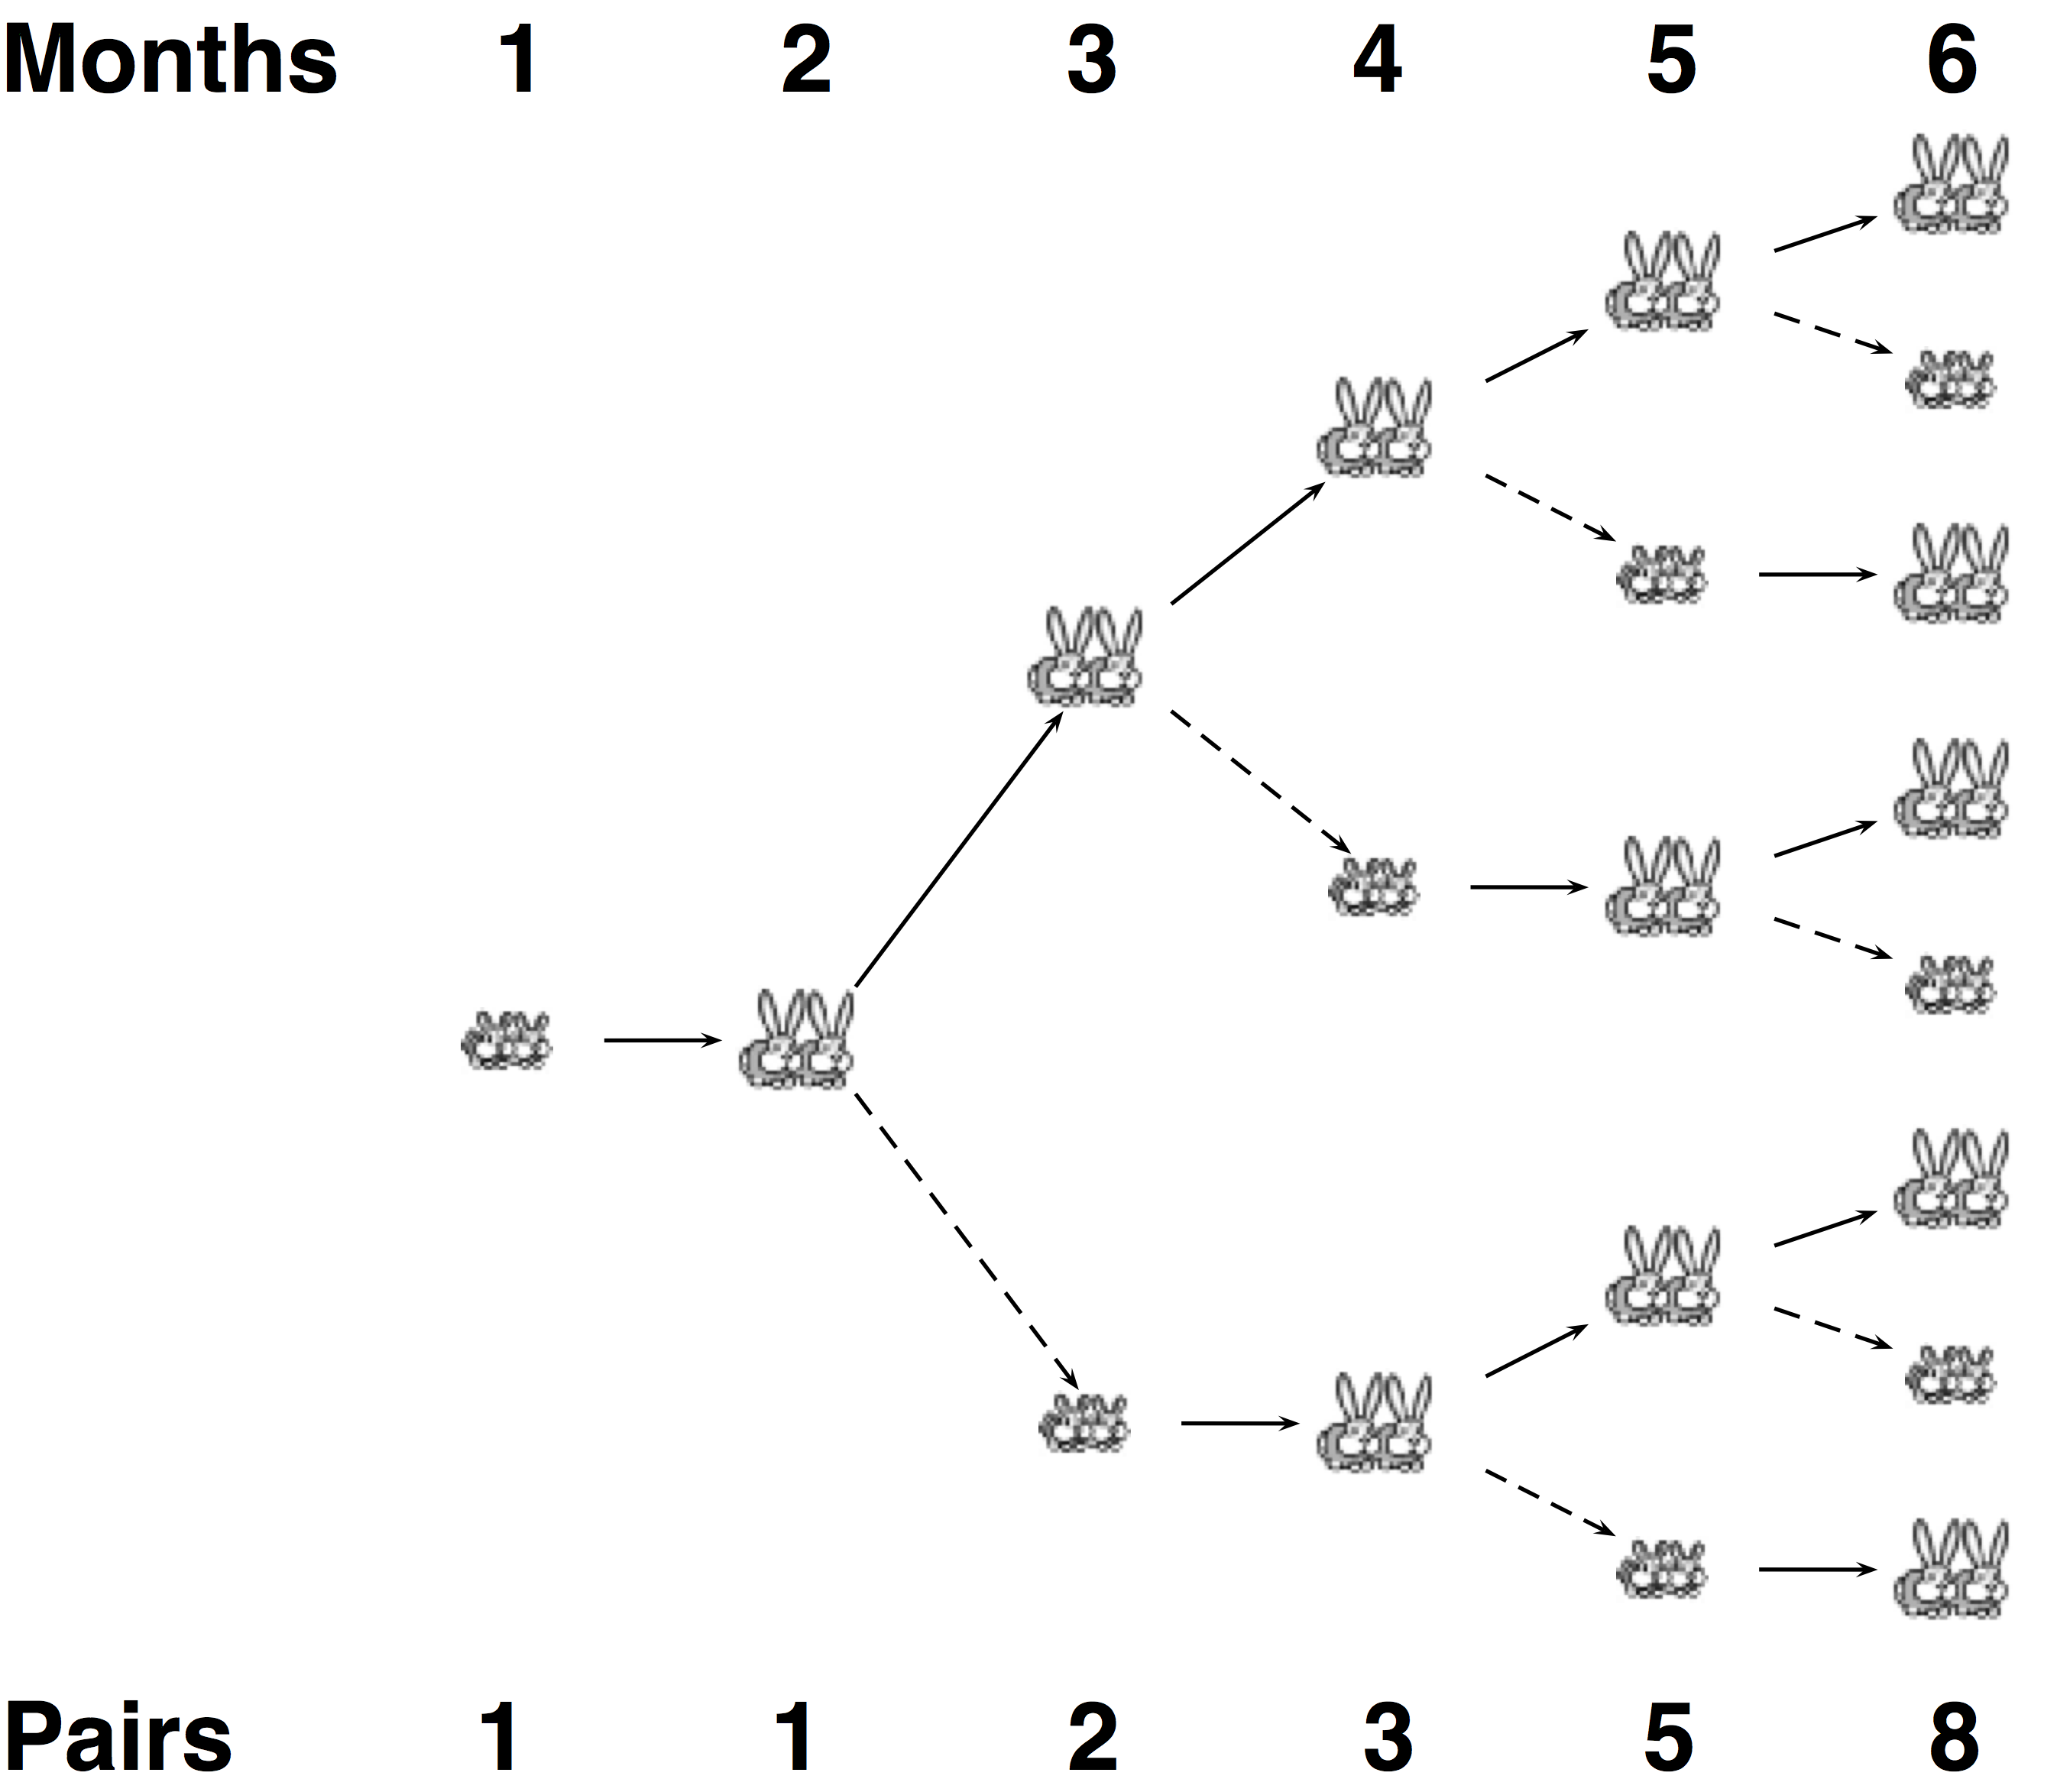
\includegraphics[width=7cm]{fib.png}    
\end{center}
Реализуйте функцию $fib'$, описывающую модель, в которой пара кроликов производит $k$ пар кроликов(в классической модели $k=1$). \\
$fib'$ --- функция двух аргументов, т.е. $fib' = \lambda kn.(\ldots)$.\\
Обычные числа Фибоначчи $fib$ можно получить так:
\[
    fib = fib'\: 1
\]
Пример: для пятого месяца ($n=5$) при $k=3$ число пар кроликов равно $fib'\: 3 \:5 = 19$
\hfill\break

Такая модель описывается уравнениями:
\begin{align*}
    fib'_k (1) &= fib'_k (2) = 1 \\
    fib'_k (n + 1) &= fib'_k (n) + k \cdot fib'_k(n - 1)
\end{align*}

Запишем функцию в лямбда исчислении:
\begin{align*}
    fib' &= \lambda kn.\operatorname{IF} \: (\LE n \: 2) \: 1 \: (\ADD \: (fib' \: k \: (\PREV n)) 
    (\MULT k \: (fib' \: k \: (\PREV (\PREV n)))) \\
    fib' &= [\lambda fkn.\operatorname{IF} \: (\LE n \: 2) \: 1 \: (\ADD \: (f \: k \: (\PREV n)) 
    (\MULT k \: (f \: k \: (\PREV (\PREV n)))) ] fib' \\
    fib' &= Y \: [\lambda fkn.\operatorname{IF} \: (\LE n \: 2) \: 1 \: (\ADD \: (f \: k \: (\PREV n)) 
    (\MULT k \: (f \: k \: (\PREV (\PREV n)))) ] 
\end{align*}


\z Покажите/объясните, что следующее выражение представляет собой комбинатор
неподвижной точки :
\[
\nsymbl{\pounds}{26}
\]
где
\[
\pounds \eqdef \lambda abcdefghijklmnopqstuvwxyzr.r(thisisafixedpointcombinator)
\]
\hfill\break

Пусть $A^n = AA...A$ -- $n$ раз записанный терм $A$ 
(это только сокращение записи, а не апликация, скобки в данной конструкции 
будут расставлены в зависимости от того, куда это выражение подставить). 
Тогда требуется доказать, что $\pounds^{26}$ - комбинатор неподвижной точки.
\begin{align*}
    \pounds^{26}f &=  (\lambda abcdefghijklmnopqstuvwxyzr.r(thisisafixedpointcombinator))\pounds^{25}f \\
    &=_\beta (\lambda r.r(\pounds^{26}r))f \\
    &=_\beta f(\pounds^{26}f)
\end{align*}

Вторая строчка верна, потому что в ``abcdefghijklmnopqstuvwxyz'' -- 25 символов, 
а в ``thisisafixedpointcombinato'' -- 26 символов (и все из них содержатся в ``abcdefghijklmnopqstuvwxyz'').
\hfill\break


\z Нарисуйте $\beta$-редукционный граф $G_\beta(M)$ для терма:
\[
M \equiv (\lambda x.\mathbf{I}xx)(\lambda x.\mathbf{I}xx) 
\]
\hfill\break


\begin{center}
    \begin{tikzpicture}[scale=1.9]
        \tikzstyle{every node}=[draw,circle,fill=black,minimum size=4pt, inner sep=0pt]
        \node[label=$M$](1) at (0pt, 0pt){};
        \node[label=right:$(\lambda x.xx)(\lambda x.Ixx)$](2) at (50pt, 0pt){};
        \node[label=right:$\omega\omega$](3) at (0pt, 50pt){};
        \node[label=above right:$(\lambda x.Ixx)(\lambda x.xx)$](4) at (-50pt, 0pt){};
        \node[label=$I\omega\omega$](5) at (-100pt, 0pt){};
        \node[label=left:$I(\lambda x.Ixx)(\lambda x.xx)$](6) at (-50pt, -50pt){};
        \node[label=below right:$I(\lambda x.Ixx)(\lambda x.Ixx)$](7) at (0pt, -50pt){};
        \node[label=right:$I(\lambda x.xx)(\lambda Ix.xx)$](8) at (50pt, -50pt){};
        
        \path[->, >=latex]
                (1)     edge [bend right]   (2)
                        edge [bend right]   (7)
                        edge                (4)
                (2)     edge [bend right]   (1)
                        edge                (3)
                (3)     edge [loop above]   (3)
                (4)     edge                (3)
                        edge                (5)
                (5)     edge                (3)
                (6)     edge                (4)
                        edge                (5)
                (7)     edge [bend right]   (1)
                        edge                (6)
                        edge                (8)    
                (8)     edge                (2)
                        edge[out=270,in=270](5);
    \end{tikzpicture}
\end{center}

\z Приведите пример замкнутого $\lambda$-терма находящегося:

$\bullet \: $ в слабой головной нормальной форме, но не в головной нормальной форме;
$$
    \lambda x.(\lambda t.t)x
$$

$\bullet \: $ в головной нормальной форме, но не в нормальной форме;
$$
    \lambda x.x((\lambda t.t)x)
$$
\hfill\break

\zopt Найдите терм, имеющий $\beta$-редукционный граф: \medskip
\[
\xymatrix{
&\bullet \ar[dr] \ar@(ul,ur)[]&\\
\bullet \ar[ur] \ar@(dl,ul)[] && \bullet \ar[dl] \ar@(ur,dr)[]\\
&\bullet  \ar[ul] \ar@(dr,dl)[]&\\
}
\]
\medskip

Искомый терм:
$$
    (\omega\omega)((\lambda abcd.ddddd)(\lambda abcd.ddddd)(\lambda abcd.ddddd)(\lambda abcd.ddddd)(\lambda abcd.ddddd))
$$
\hfill\break

\zopt Докажите, что:
\[\forall M \in \Lambda, \exists N \in \Lambda: N\mathbf{I} \twoheadrightarrow_\beta M 
\]
 где терм $N$ в $\beta$-нормальной форме.
\hfill\break

Пройдемся по $M$ и заменим все редексы $((\lambda t.X)Y)$ на $(x(\lambda t.X)Y)$, где $x \not\in FV(M)$.
Тогда все редексы нейтрализуются, а новых не появится, значит полученый терм $M'$ будет в нормальной форме.
Искомый терм $N$ можно выразить как $N \equiv \lambda x.M'$.

\end{document}